\subsubsection{Ingress}

Ein Kubernetes-Cluster kann, wenn er Daten von außen benötigt, diese einfach abrufen. Wenn jedoch eine Anwendung im Cluster außerhalb des Clusters erreichbar sein soll, muss dies zuerst eingerichtet werden.

Wenn nur eine TCP-Verbindung benötigt wird, kann ein Service vom Typ NodePort erhalten werden. Wenn jedoch eine HTTP-Verbindung benötigt wird, wird ein Ingress benötigt.

Ein Ingress erhält dabei die Anfrage von außen und leitet sie an den passenden Service weiter. Dies kann über den Host oder den Pfad einer URL entschieden werden.
Über den Ingress können auch TLS-Zertifikate eingefügt werden, um HTTPS-Verbindungen zu erstellen.
\begin{figure}[htbp]
\centering
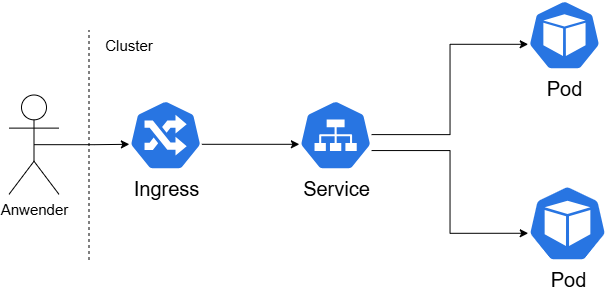
\includegraphics[width=0.8\textwidth]{bilder/grundlagen/kommunikation.png}
\caption{Kommunikation mit Ingress und Service}
\label{fig:kommunikation}
\end{figure}
\FloatBarrier